% % !TEX root = ../Thesis.tex
% \chapter{Demonstration and Evaluation} 
% \label{cha:Evaluation}




% \section{Demonstration of the Artefact}


% The artefact was demonstrated using real workflow data from the year 2024 calculation cycle in order to evaluate its implemented workflow stages and inspectable outputs. The demonstration covered the deployed prototype setting, execution of the workflow in the web-based environment, and validation of selected outputs against manually verified 2024 results.


% \subsection{Setup of Test Environment}



% For the demonstration, the artefact was operated as a browser-accessible prototype in a \textit{controlled deployment environment}. The frontend, backend, and database layer were run together as one integrated web-based system, allowing users to access the workflow through the implemented interface rather than through local development views alone.

% The evaluation dataset consisted of real workflow data from the \textit{2024 calculation cycle}. This included OTH data, CRP and SAL related reference data, Volvo CE sales data, and matrix-based business input such as source matrix together with related mapping files. These datasets were used as the input basis for evaluating the implemented \textit{preparation}, \textit{adjustment}, and \textit{split-related} logic.


% % \subsection{Execution with Uploaded Workflow Data}

% % In the demonstration, source matrix CSV, CRP and SAL CSV files, and OTH CSV files were submitted through the implemented upload pages of the prototype. The uploaded files were processed successfully and could be displayed again through the corresponding frontend views and report tables.

% % This execution step showed that the prototype could handle heterogeneous CSV input in a consistent way. The implemented parsing logic supported normalization of column names and values, recognition of different header styles, handling of repeated header-like rows, and correct assignment of uploaded values to the expected workflow columns. As a result, the uploaded rows could be aligned reliably with the internal report structure used in later workflow stages.

% % The processed data was then available through filterable tables in the frontend, where rows and columns could be inspected directly. In addition, the prototype supported CSV download of complete generated result tables, allowing the exported outputs to be checked outside the web interface.



% % \subsection{Execution with Uploaded Workflow Data}

% % In the demonstration, the required workflow inputs were uploaded through the implemented frontend pages, including Source Matrix CSV, Reporter List CSV, Size Class CSV, Brand Mapping CSV, Group Country CSV, Machine Line Mapping CSV, OTH data, and CRP-related data. The upload views showed the availability of the required input categories, and each upload could be followed by showing the latest stored version or downloading the latest file from the interface.

% % The uploaded 2024 files were displayed correctly after submission, and the downloaded files matched the expected content without formatting issues or character corruption. The prototype also allowed edited upload data to be saved and downloaded again, and the resulting files remained consistent with the expected output. This confirmed that the upload, display, download, and save functionality worked correctly for the tested 2024 workflow inputs.

% % For the uploaded OTH and CRP data, the cleaned outputs were compared with the corresponding 2024 SAP export tables. The SQL-based cleaning and matching logic produced the expected values, including correct alignment of fields such as country name and market area. The comparison showed that the generated tables were consistent with the SAP reference data, indicating that the upload and initial data-processing steps behaved as intended within the scope of the evaluation.



% \subsection{Execution with Uploaded Workflow Data}

% After the test environment had been prepared, the prototype was executed with the selected 2024 TMC workflow data. The execution followed the implemented workflow sequence from file upload and backend processing to preparation, adjustment, market-view generation, split/resplit processing, and output review.

% The generated outputs were presented through filterable tables, summary views, charts, and CSV export functions. Table~\ref{tab:execution_outputs} summarises the execution steps and main outputs.

% \begin{longtable}{|>{\raggedright\arraybackslash}p{1.0cm}|>{\raggedright\arraybackslash}p{4.6cm}|>{\raggedright\arraybackslash}p{7.8cm}|}
% \caption{Execution flow and main outputs}
% \label{tab:execution_outputs} \\
% \hline
% \textbf{Step} & \textbf{Execution Activity} & \textbf{Main Output Produced} \\
% \hline
% \endfirsthead

% \hline
% \textbf{Step} & \textbf{Execution Activity} & \textbf{Main Output Produced} \\
% \hline
% \endhead

% 1 & Upload source and matrix files & Stored workflow inputs, including Source Matrix, Reporter List, Size Class, Brand Mapping, Group Country, and Machine Line Mapping, with display and download functions. \\
% \hline

% 2 & Upload and register CRP/TMA/SAL/OTH input data & Stored CRP- and TMA-related files, Volvo Sales data, and OTH data as executable workflow inputs for downstream stages. \\
% \hline

% 3 & Generate OTH deletion and reporter base input & Row-level OTH base records with deletion indicators, reporter indicators, source-related fields, and summary values. \\
% \hline

% 4 & Run preparation-stage processing & Cleaned, mapped, and aggregated preparation outputs with mapped dimensions, reporter/deletion fields, and stage-level intermediate results. \\
% \hline

% 5 & Generate market-view and VCE / Non-VCE results & Market-view outputs showing Total Market, Volvo CE, Non-Volvo CE values, summary cards, and ratio-related values. \\
% \hline

% 6 & Run adjustment-stage processing & Adjustment-layer tables with grouped and derived values for intermediate workflow review. \\
% \hline

% 7 & Execute split and resplit logic & Split and resplit outputs with split level, split ratio, before/after values, redistributed rows, and case-related results. \\
% \hline

% 8 & Inspect and export outputs & Filterable stage views, summary views, chart-based review, and CSV export files for comparison and evaluation. \\
% \hline

% \end{longtable}

% % This execution demonstrated how the prototype moves from uploaded source and matrix files to staged preparation, adjustment, split, and export outputs. The generated outputs were then used as the basis for the validation and requirement-based evaluation in the following sections.

% % \section{Evaluation of the Artefact}


% % The artefact was evaluated against the requirements defined in Section~\ref{sec:requirements}. The evaluation assessed both the correctness of the generated outputs and the extent to which the prototype fulfilled the functional, structural, performance, quality, and environmental requirements.

% % The evaluation therefore combined output validation with requirement-based assessment. The generated results were checked against expected business rules and, where comparable, 2024 SAP reference outputs. The requirement-based assessment focused on transparency, traceability, usability, validation support, and prototype-level performance within the selected workflow scope.


% % \subsection{Validation of Prototype Outputs}

% % The generated prototype outputs were validated against the expected workflow logic and, where comparable, against 2024 SAP reference outputs. This validation focused on whether the SQL-based processing produced correct cleaned, mapped, aggregated, split, and resplit-related outputs within the implemented workflow scope.

% % For the preparation stage, validation focused on row counts, mapped fields, reporter and deletion-related flags, aggregated values, and VCE / Non-VCE market-view calculations. For the split and resplit stages, validation focused on whether the prototype identified the correct split records, assigned the expected split levels and split ratios, redistributed values according to the defined business rules, and preserved before- and after-split totals. The detailed validation results are presented in the following subsections.






% % % \subsection{Preparation-Stage Validation}

% % % The preparation stage was evaluated by comparing the generated prototype outputs with workflow data from the 2024 calculation cycle that had already been manually checked. 

% % % For the CRP/TMA- and sales-related preparation outputs, the comparison examined whether the implemented preparation logic produced the expected workflow control fields and grouped values. In particular, the generated deletion flag and reporter flag were checked against the corresponding verified 2024 reference results. The comparison showed that these preparation-related outputs were consistent with the manually verified 2024 data.

% % % For OTH-related preparation, the evaluation focused on whether uploaded source rows were correctly aligned with the relevant mapping structures and then aggregated into the expected preparation-level outputs. In this stage, the mapped OTH values, including brand-related aggregated results, were displayed in the frontend tables and compared with the corresponding manually verified 2024 reference data. The comparison confirmed that the implemented OTH mapping and aggregation logic produced results consistent with the verified 2024 outputs.

% % % The preparation-stage evaluation also included inspection of the frontend-based market-view representation. The VCE and Non-VCE chart was rendered correctly and displayed the expected percentage distribution between the two value categories. In addition, the chart and summary values responded correctly to frontend filtering, and the displayed percentages and totals remained consistent with the filtered result set.


% % % \subsection{Validation of Adjustment- and Split-Related Results}

% % % After the preparation-stage outputs had been validated, the adjustment- and split-related results were evaluated through comparison with manually verified 2024 reference data. This validation focused on whether the implemented later-stage workflow logic produced outputs consistent with the expected 2024 results.

% % % For the adjustment stage, the generated output was compared with the corresponding manually verified 2024 result structure. The comparison showed that the grouped values, source-detail rows, and derived result rows generated by the prototype were consistent with the expected adjustment-related outputs within the scope of the implementation. The frontend representation also allowed these result rows to be inspected directly, making it possible to review how the adjustment output had been formed.

% % % For the split-related stage, validation focused on whether grouped values were redistributed into the expected more detailed result structures. In particular, the evaluation examined the calculated split ratios and the resulting redistributed values. These were compared with the corresponding manually verified 2024 split results. The comparison indicated that the implemented split ratios and the resulting split outputs were consistent with the expected reference results within the scope of the prototype.

% % % The split-related frontend views also supported direct inspection of both summary rows and detailed split rows, including the values before and after redistribution. 


% % % \subsection{Validation of Split- and Resplit-Related Results}

% % % The split- and resplit-related functionality was validated in two steps. First, the number of rows requiring split in the Excavators Split Case and Wheel Loaders Split Case was calculated and compared with the corresponding 2024 SAP records. This check was used to confirm that the prototype identified the same machine-line records as the reference system. In the tested cases, the resulting split row counts and machine-line assignments were consistent with the 2024 SAP outputs.

% % % Second, approximately 20\% of the resulting rows were manually spot-checked in more detail. For these sampled records, the Split Level and Split Ratio values were compared with the corresponding SAP-generated records and with the expected values defined by the split rules. The comparison showed that the prototype produced values consistent with both the SAP reference data and the defined business rules.

% % % Overall, the evaluation indicated that the split and resplit logic behaved as expected within the scope of the tested 2024 cases. The generated outputs matched the reference records, and the detailed sampled checks confirmed that the redistributed values followed the intended split definitions.




% % % \subsection{Preparation-Stage Validation}

% % % The preparation stage was validated by comparing the generated prototype outputs with the corresponding 2024 SAP reference data. The evaluation focused on whether the cleaned and mapped preparation outputs preserved the expected workflow structure, correctly assigned the relevant control fields, and produced row counts and aggregated values consistent with the reference system.

% % % For the CRP-related preparation output, the prototype was checked against the expected reporter classification and grouped preparation structure. In the tested 2024 data, the number of CRP rows identified as reporter rows was 338, which matched the corresponding SAP reference result. In addition, the deletion-related logic was checked to ensure that rows flagged for exclusion were treated consistently with the SAP output.

% % % For the OTH-related preparation output, the cleaned rows were compared with the SAP export to verify that the mapping logic produced the expected field values. In particular, fields such as country name and market area were checked against the corresponding SAP-generated tables, and the resulting outputs were found to be consistent. The evaluation also confirmed that the OTH Reporter Flag was assigned correctly, with 3,407 rows matching the expected reporter classification in the tested 2024 data.

% % % The preparation-stage validation also included the generated VCE / Non-VCE market view. Approximately 20\% of the resulting rows were manually spot-checked to verify that, for each tested country and machine-line combination, the TMA value was correctly reduced by the corresponding Volvo sales value and that the resulting VCE / Non-VCE ratio was displayed correctly. The checked records were consistent with the expected calculations, confirming that the prototype produced the intended market-share representation for the tested 2024 data.

% % % Overall, the preparation-stage validation showed that the prototype produced cleaned, mapped, and aggregated outputs consistent with the 2024 SAP reference data. The row counts, control flags, key mapped fields, and market-view calculations all matched the expected values, indicating that the implemented preparation logic behaved correctly within the scope of the evaluation.

% % \subsection{Preparation-Stage Validation}

% % The preparation stage was evaluated through data comparison and output inspection. The purpose of this validation was to assess whether the prototype generated preparation outputs that were consistent with the expected workflow logic and the corresponding 2024 SAP reference data. The evaluation parameters included row-count consistency, correctness of mapped fields, correctness of workflow control flags, and correctness of the VCE / Non-VCE market-view calculation.

% % For the CRP-related preparation output, the prototype result was compared with the expected reporter classification and grouped preparation structure from the SAP reference data. In the tested 2024 data, the number of CRP rows identified as reporter rows was 338, which matched the corresponding SAP reference result. The deletion-related logic was also checked to verify that rows flagged for exclusion were treated consistently with the SAP output.

% % For the OTH-related preparation output, the cleaned and mapped rows were compared with the SAP export tables. The comparison focused on whether key mapped fields, such as country name and market area, were aligned with the SAP-generated values. The generated outputs were consistent with the SAP reference data. The OTH Reporter Flag was also assigned correctly, with 3,407 rows matching the expected reporter classification in the tested 2024 data.

% % The preparation-stage validation further included the generated VCE / Non-VCE market view. Approximately 20\% of the resulting rows were manually spot-checked across selected country and machine-line combinations. For each checked record, the validation examined whether the TMA value was correctly reduced by the corresponding Volvo CE sales value and whether the resulting VCE / Non-VCE ratio was displayed correctly. The checked records were consistent with the expected calculations.



% % % \subsection{Validation of Split- and Resplit-Related Results}

% % % The split- and resplit-related functionality was validated in two steps. First, the number of rows requiring split in the Excavators Split Case and Wheel Loaders Split Case was calculated and compared with the corresponding 2024 SAP records. This check was used to verify that the prototype identified the same machine-line records as the reference system. In the tested cases, the resulting split row counts and machine-line assignments were consistent with the 2024 SAP outputs.

% % % Second, approximately 20\% of the resulting rows were manually spot-checked in more detail. The sampled records were selected from different country and machine-line combinations to ensure that the validation covered representative split patterns. For each sampled row, the Split Level, Split Ratio, and redistributed values were compared with both the SAP-generated records and the expected values defined by the split rules. In addition, the before-split and after-split values were checked to confirm that the redistribution followed the intended business logic and preserved the original totals.

% % % The same validation approach was applied to the resplit functionality. In this case, the resplit logic was guided by a manual business-rule check of whether a brand was actually sold in the relevant country or region for the affected machine line. If one of the finer target categories did not exist for that brand in the given market, the corresponding value was reassigned to the remaining valid category. In practice, the resplit logic redistributed the value into two finer buckets, ensuring that the value of the missing bucket was moved to the existing one according to the resplit rules. A similar spot-check was then applied to approximately 20\% of the resplit rows. The sampled records were compared with the corresponding SAP outputs and with the expected business-rule outcome for the relevant brand and region, and the results were consistent in the tested cases.

% % % Overall, the evaluation showed that the prototype produced split and resplit outputs consistent with the 2024 SAP reference data. The row selection, split assignment, and redistribution logic were consistent with the expected machine-line records, and the sampled detailed checks confirmed that the implemented behaviour matched the business rules within the scope of the tested cases.




% % \subsection{Split- and Resplit-Related Validation}

% % The split- and resplit-related outputs were evaluated through comparison with 2024 SAP reference records and manual output inspection. The validation focused on four parameters: correct identification of records requiring split, correctness of split level and split ratio assignment, correctness of redistributed values, and preservation of before- and after-split totals.

% % For the split functionality, the number of rows requiring split in the Excavators Split Case and Wheel Loaders Split Case was calculated and compared with the corresponding 2024 SAP records. This check verified whether the prototype identified the same machine-line records as the reference system. In the tested cases, the split row counts and machine-line assignments were consistent with the SAP outputs. Approximately 20\% of the resulting split rows were then manually spot-checked across different country and machine-line combinations. For each sampled row, the split level, split ratio, redistributed values, and before- and after-split totals were compared with the SAP-generated records and the expected values defined by the split rules.

% % The same validation approach was applied to the resplit functionality. The resplit logic was checked against the business rule that invalid brand--machine-line--size-class combinations should be removed and redistributed to the remaining valid categories. Approximately 20\% of the resplit rows were manually spot-checked and compared with the corresponding SAP outputs and expected business-rule outcomes. The sampled results were consistent in the tested cases, indicating that the implemented split and resplit logic behaved correctly within the evaluated scope.

% % During the split validation, one discrepancy was also observed between the currently expected split logic and the corresponding SAP output. According to the business interpretation used in the prototype, machine-line split for non-VCE reporter-brand values should be based on the distribution of non-VCE TMA values across the relevant finer size classes. Since the split is applied to non-VCE values, Volvo CE volume should be excluded from TMA before calculating the split ratio. However, in one reviewed SAP case, the observed split ratio appeared to be calculated from total TMA values including Volvo CE volume. This produced a different allocation compared with the non-VCE-based split ratio implemented in the prototype.

% % This discrepancy suggests that the SAP output may reflect historical calculation logic or an implementation detail that is not fully aligned with the currently expected business rule. It was therefore not treated simply as a prototype error, but as an important validation finding. The case demonstrates how making intermediate split ratios and rule applications visible can support discussion and clarification of business rules that are otherwise difficult to inspect in the SAP-based workflow.



% \section{Evaluation of the Artefact}

% The artefact was evaluated against the requirements defined in Section~\ref{sec:requirements}. The evaluation combined output validation with requirement-based assessment. Output validation examined whether the generated results were consistent with expected business rules and, where comparable, with 2024 SAP reference outputs. Requirement-based assessment examined whether the prototype fulfilled the functional, structural, performance, quality, and environmental requirements, with particular attention to transparency, traceability, usability, validation support, and prototype-level performance.

% \subsection{Validation of Prototype Outputs}

% The generated prototype outputs were validated against the expected workflow logic and, where comparable, against 2024 SAP reference outputs. The validation used comparison-based parameters to assess whether the SQL-based processing produced correct cleaned, mapped, aggregated, split, and resplit-related outputs within the implemented workflow scope.

% For the preparation stage, the validation parameters were:
% \begin{itemize}
%     \item row-count consistency;
%     \item mapped-field consistency;
%     \item workflow control-flag correctness;
%     \item aggregated-value consistency;
%     \item correctness of the VCE / Non-VCE market-view calculation.
% \end{itemize}

% For the split and resplit stages, the validation parameters were:
% \begin{itemize}
%     \item correct identification of records requiring split;
%     \item correctness of split level and split ratio assignment;
%     \item correctness of redistributed values;
%     \item preservation of before- and after-split totals.
% \end{itemize}

% The detailed validation results are presented in the following subsections.

% \subsection{Preparation-Stage Validation}

% The preparation stage was evaluated through comparison with 2024 SAP reference data and manual output inspection. The purpose was to assess whether the generated preparation outputs were consistent with the expected workflow logic.

% For the CRP-related preparation output, the prototype result was compared with the expected reporter classification and grouped preparation structure from the SAP reference data. In the tested 2024 data, 338 CRP rows were identified as reporter rows, matching the corresponding SAP reference result. The deletion-related logic was also checked to verify that rows flagged for exclusion were treated consistently with the SAP output.

% For the OTH-related preparation output, the cleaned and mapped rows were compared with SAP export tables. Key mapped fields, such as country name and market area, were aligned with the SAP-generated values. The OTH Reporter Flag was also assigned correctly, with 3,407 rows matching the expected reporter classification in the tested 2024 data.

% The preparation-stage validation further included the generated VCE / Non-VCE market view. Approximately 20\% of the resulting rows were manually spot-checked across selected country and machine-line combinations. For each checked record, the validation examined whether the TMA value was correctly reduced by the corresponding Volvo CE sales value and whether the resulting VCE / Non-VCE ratio was displayed correctly. The checked records were consistent with the expected calculations.

% Overall, the preparation-stage validation showed that the prototype produced cleaned, mapped, and aggregated outputs consistent with the 2024 SAP reference data and expected business logic within the tested scope.

% \subsection{Split- and Resplit-Related Validation}

% The split- and resplit-related outputs were evaluated through comparison with 2024 SAP reference records and manual output inspection. The validation focused on split-record identification, split-level and split-ratio correctness, redistributed-value correctness, and preservation of before- and after-split totals.

% For the split functionality, the number of rows requiring split in the Excavators Split Case and Wheel Loaders Split Case was calculated and compared with the corresponding 2024 SAP records. This check verified whether the prototype identified the same machine-line records as the reference system. In the tested cases, the split row counts and machine-line assignments were consistent with the SAP outputs. Approximately 20\% of the resulting split rows were then manually spot-checked across different country and machine-line combinations. For each sampled row, the split level, split ratio, redistributed values, and before- and after-split totals were compared with the SAP-generated records and the expected values defined by the split rules.

% The same validation approach was applied to the resplit functionality. The resplit logic was checked against the business rule that invalid brand--machine-line--size-class combinations should be removed and redistributed to the remaining valid categories. Approximately 20\% of the resplit rows were manually spot-checked and compared with the corresponding SAP outputs and expected business-rule outcomes. The sampled results were consistent in the tested cases, indicating that the implemented split and resplit logic behaved correctly within the evaluated scope.

% \paragraph{Observed discrepancy in split logic.}
% During the split validation, one discrepancy was also observed between the currently expected split logic and the corresponding SAP output. According to the business interpretation used in the prototype, machine-line split for non-VCE reporter-brand values should be based on the distribution of non-VCE TMA values across the relevant finer size classes. Since the split is applied to non-VCE values, Volvo CE volume should be excluded from TMA before calculating the split ratio. However, in one reviewed SAP case, the observed split ratio appeared to be calculated from total TMA values including Volvo CE volume. This produced a different allocation compared with the non-VCE-based split ratio implemented in the prototype.

% This discrepancy suggests that the SAP output may reflect historical calculation logic or an implementation detail that is not fully aligned with the currently expected business rule. It was therefore not treated simply as a prototype error, but as an important validation finding. The case demonstrates how making intermediate split ratios and rule applications visible can support discussion and clarification of business rules that are otherwise difficult to inspect in the SAP-based workflow.



% \section{Evaluation Against Requirements}

% The artefact was further evaluated against the requirements defined in Section~\ref{sec:requirements}. To make the assessment explicit, each requirement was linked to an evaluation parameter or metric and evaluated using evidence from the prototype functions, generated outputs, validation checks, and stakeholder feedback.

% SAP reference outputs were used where direct comparison was possible, particularly for validating preparation-, split-, and resplit-related results. However, not all evaluation parameters could be assessed through direct SAP comparison. Transparency, traceability, and usability were evaluated mainly through the implemented prototype functions, the visibility of intermediate outputs, the availability of source and rule context fields, and stakeholder feedback during prototype review. Performance and stability were assessed at prototype level through observed execution and repeated review operations in the test environment.

% The results are summarised in Table~\ref{tab:evaluation_parameters}.

% \begin{longtable}{|>{\raggedright\arraybackslash}p{1.2cm}|>{\raggedright\arraybackslash}p{2.7cm}|>{\raggedright\arraybackslash}p{4.0cm}|>{\raggedright\arraybackslash}p{6.0cm}|}
% \caption{Evaluation against requirements}
% \label{tab:evaluation_parameters} \\
% \hline
% \textbf{ID} & \textbf{Evaluation Dimension} & \textbf{Evaluation Parameter / Metric} & \textbf{Evidence and Evaluation Result} \\
% \hline
% \endfirsthead

% \hline
% \textbf{ID} & \textbf{Evaluation Dimension} & \textbf{Evaluation Metric} & \textbf{Evidence and Evaluation Result} \\
% \hline
% \endhead

% FR1 & Functional fulfilment & Completion of source and matrix file upload and management. & CSV-based source data and matrix files were uploaded through the frontend pages. The uploaded files could be displayed, stored, downloaded, and reused in later workflow stages. \\
% \hline

% FR2 & Functional fulfilment & Successful execution of backend workflow processing. & Backend processing re-expressed selected SAP-based TMC workflow logic, including preparation, adjustment, and split-related processing. The generated outputs were used for validation against expected business rules and, where comparable, SAP reference outputs. \\
% \hline

% FR3 & Functional fulfilment / usability & Availability of frontend review functions. & The prototype provided filterable tables, summary values, chart-based review, and CSV export. These functions allowed users to inspect detailed records and aggregated outputs through the browser interface. \\
% \hline

% SR1 & Structural fit & Separation of upload, processing, storage, and visualisation components. & The artefact used a modular web-based frontend-backend architecture, with frontend views, backend services, and relational database storage separated into different components. \\
% \hline

% SR2 & Structural fit & Structured storage of uploaded files, mappings, workflow records, and generated outputs. & Uploaded files, mapping data, intermediate workflow records, and generated outputs were stored in structured form, supporting repeated review and future extension to later workflow stages. \\
% \hline

% PR1 & Performance & Successful completion of stage and report execution for the selected 2024 dataset. & Demonstration runs using the selected 2024 TMC data completed within a practically acceptable time for prototype-based review. Formal production-level benchmarking was outside the thesis scope. \\
% \hline

% PR2 & Performance / stability & Absence of crashes, data loss, or inconsistent save/reload behaviour during repeated operations. & Repeated upload, processing, filtering, save/reload, and export operations were performed in the test environment. The prototype remained usable for prototype-level evaluation. \\
% \hline

% QR1 & Transparency & Visibility of intermediate workflow stages, row-level outputs, and stage summaries. & Compared with the SAP-based representation, the prototype exposed preparation, adjustment, split, and resplit-related outputs as separate inspectable stages. Row-level tables and summaries allowed users to review how values were formed step by step within the implemented scope. \\
% \hline

% QR2 & Traceability & Availability of source, mapping, control-flag, and rule-decision context in generated stage outputs. & Generated outputs preserved relevant stage-level context, including source, country, machine line, brand, reporter flags, deletion flags, split levels, and split ratios. This supported stage-level traceability between input data, rule context, and generated outputs, while full row-level lineage remains future work. \\
% \hline

% QR3 & Usability & Ability to complete BI review tasks through the browser interface with acceptable effort. & Users could navigate workflow stages, inspect records, filter outputs, review summaries and charts, and export CSV files. Stakeholder feedback indicated that these functions were useful for review and validation tasks, although further interface refinement would be needed for broader operational use. \\
% \hline

% ER1 & Environmental fit & Operation in a controlled prototype environment. & The artefact was operated as a browser-accessible prototype using a web frontend, backend service, and relational database. This environment supported demonstration and evaluation with the selected 2024 workflow data. \\
% \hline

% ER2 & Environmental fit & Future adaptability to more robust cloud or Volvo CE internal infrastructure. & The modular architecture provides a basis for future adaptation to more robust cloud deployment or Volvo CE internal infrastructure. Full enterprise integration remains future work. \\
% \hline

% \end{longtable}




% \section{Comparison with the SAP-Based Workflow}

% To further clarify the evaluation of transparency, traceability, usability, validation support, and performance, the prototype was compared with the current SAP-based workflow representation from a business-user perspective. This comparison does not claim that SAP lacks these capabilities technically. Rather, it assesses whether the functions are directly available and inspectable for business users within the reviewed workflow.

% \begin{longtable}{|
% >{\raggedright\arraybackslash}p{2.6cm}|
% >{\raggedright\arraybackslash}p{2.4cm}|
% >{\raggedright\arraybackslash}p{2.4cm}|
% >{\raggedright\arraybackslash}p{6.2cm}|}
% \caption{Comparison between the SAP-based workflow and the prototype from a business-user perspective}
% \label{tab:sap_prototype_comparison} \\
% \hline
% \textbf{Evaluation Dimension} & \textbf{SAP-based Workflow} & \textbf{Prototype} & \textbf{Explanation} \\
% \hline
% \endfirsthead

% \hline
% \textbf{Evaluation Dimension} & \textbf{SAP-based Workflow} & \textbf{Prototype} & \textbf{Explanation} \\
% \hline
% \endhead

% Transparency & Limited for business users & Supported & The prototype exposes preparation, adjustment, split, and resplit outputs as separate inspectable stages. In the SAP-based representation, these workflow layers are not provided in one review-oriented interface for business users. \\
% \hline

% Traceability & Limited for business users & Partly supported & The prototype preserves stage-level source and rule context fields, such as country, machine line, source, brand, flags, split level, and split ratio. Full row-level lineage across all transformations is not yet implemented. \\
% \hline

% Usability & Limited for business users & Supported & The prototype provides browser-based filtering, summaries, chart-based review, and CSV export for BI review tasks. The SAP-based workflow requires more SAP-specific navigation and technical knowledge. \\
% \hline

% Validation support & Limited for business users & Supported & Intermediate outputs, totals, flags, and split ratios can be inspected and compared with expected business rules in the prototype. In the SAP-based workflow, such validation often requires additional extraction or IT-supported investigation. \\
% \hline

% Performance and stability & Not directly compared & Prototype-level support & The prototype completed the selected 2024 workflow runs and remained usable during repeated upload, processing, filtering, save/reload, and export operations. A direct production-level performance comparison with SAP was outside the thesis scope. \\
% \hline

% \end{longtable}














% % \section{Evaluation Against Requirements}

% % The implemented artefact was assessed in relation to the requirements identified in Chapter 4. The outcome of this assessment is summarized in Table 4.1.

% % \begin{table}[H]
% % \centering
% % \begin{tabular}{p{2.5cm} p{10cm}}
% % \hline
% % \textbf{Category} & \textbf{Evaluation Result} \\
% % \hline

% % \textbf{Functional} & The artefact supports structured upload and management of CSV-based source data and matrix files, allowing users to provide the required inputs for the workflow. \\

% % \textbf{Functional} & Key parts of the SAP-based workflow logic were re-expressed through backend processing and staged report generation, making the transformation steps more explicit and easier to follow. \\

% % \textbf{Functional} & Within the scope of the prototype, preparation, adjustment, and split-related stages are represented through inspectable workflow-layer outputs, enabling step-by-step validation. \\

% % \textbf{Functional} & The frontend supports filtering, summary calculation, chart-based inspection, and CSV export, allowing users to explore both detailed records and aggregated results. \\

% % \hline

% % \textbf{Structural} & The artefact is implemented as a web-based system with a clear separation between frontend and backend components. \\

% % \textbf{Structural} & Upload handling, backend processing, and frontend visualization are implemented as separate modules, which improves maintainability and extensibility. \\

% % \textbf{Structural} & Within the prototype scope, the system supports structured storage of workflow data, mappings, and derived outputs, while allowing further extensions. \\

% % \hline

% % \textbf{Environmental} & The artefact provides a more transparent and user-oriented representation compared to the original SAP-based workflow. \\

% % \textbf{Environmental} & Intermediate outputs, totals, and potential data issues can be inspected directly, supporting validation and analysis. \\

% % \textbf{Environmental} & The prototype demonstrates potential for supporting market-related analysis, although full integration into existing enterprise systems remains future work. \\

% % \hline
% % \end{tabular}
% % \caption{Evaluation of artefact requirements}
% % \label{tab:requirement_evaluation_tmc}
% % \end{table}


% \section{Summary and Limitations}

% The evaluation showed that the artefact fulfills its core purpose as a web-based prototype for the TMC workflow. Within the implemented scope, the system supported structured CSV upload, staged backend processing, workflow-layer inspection, and validation of generated outputs against manually verified 2024 reference results.

% Several limitations nonetheless apply:
% \begin{itemize}
% \item The prototype covers only selected stages of the broader TMC process.
% \item The validation was conducted with data from the 2024 calculation cycle, so the results cannot yet be generalised across all years and workflow variations.
% \item The artefact remains sensitive to the structural quality of uploaded CSV files and mapping data, despite the cleaning and normalisation logic that has been implemented.
% \item The current deployment and storage setup is adequate for prototype use, but broader internal deployment would require more robust infrastructure and deeper integration with enterprise systems.
% \end{itemize}

% !TEX root = ../Thesis.tex


% \chapter{Demonstration and Evaluation} 
% \label{cha:Evaluation}

% \section{Demonstration of the Artefact}


% The artefact was demonstrated using real workflow data from the year 2024 calculation cycle in order to evaluate its implemented workflow stages and inspectable outputs. The demonstration covered the deployed prototype setting, execution of the workflow in the web-based environment, and validation of selected outputs against manually verified 2024 results.


% \subsection{Setup of Test Environment}

% For the demonstration, the artefact was operated as a browser-accessible prototype in a \textit{controlled deployment environment}. The frontend, backend, and database layer were run together as one integrated web-based system, allowing users to access the workflow through the implemented interface rather than through local development views alone.

% The evaluation dataset consisted of real workflow data from the \textit{2024 calculation cycle}. This included OTH data, CRP and SAL related reference data, Volvo CE sales data, and matrix-based business input such as source matrix together with related mapping files. These datasets were used as the input basis for evaluating the implemented \textit{preparation}, \textit{adjustment}, and \textit{split-related} logic.

% \subsection{Execution with Uploaded Workflow Data}

% After the test environment had been prepared, the prototype was executed with the selected 2024 TMC workflow data. The execution followed the implemented workflow sequence from file upload and backend processing to preparation, adjustment, market-view generation, split/resplit processing, and output review.

% The generated outputs were presented through filterable tables, summary views, charts, and CSV export functions. Table~\ref{tab:execution_outputs} summarises the execution steps and main outputs.

% \begin{longtable}{|>{\raggedright\arraybackslash}p{1.0cm}|>{\raggedright\arraybackslash}p{4.6cm}|>{\raggedright\arraybackslash}p{7.8cm}|}
% \caption{Execution flow and main outputs}
% \label{tab:execution_outputs} \\
% \hline
% \textbf{Step} & \textbf{Execution Activity} & \textbf{Main Output Produced} \\
% \hline
% \endfirsthead

% \hline
% \textbf{Step} & \textbf{Execution Activity} & \textbf{Main Output Produced} \\
% \hline
% \endhead

% 1 & Upload source and matrix files & Stored workflow inputs, including Source Matrix, Reporter List, Size Class, Brand Mapping, Group Country, and Machine Line Mapping, with display and download functions. \\
% \hline

% 2 & Upload and register CRP/TMA/SAL/OTH input data & Stored CRP- and TMA-related files, Volvo Sales data, and OTH data as executable workflow inputs for downstream stages. \\
% \hline

% 3 & Generate OTH deletion and reporter base input & Row-level OTH base records with deletion indicators, reporter indicators, source-related fields, and summary values. \\
% \hline

% 4 & Run preparation-stage processing & Cleaned, mapped, and aggregated preparation outputs with mapped dimensions, reporter/deletion fields, and stage-level intermediate results. \\
% \hline

% 5 & Generate market-view and VCE / Non-VCE results & Market-view outputs showing Total Market, Volvo CE, Non-Volvo CE values, summary cards, and ratio-related values. \\
% \hline

% 6 & Run adjustment-stage processing & Adjustment-layer tables with grouped and derived values for intermediate workflow review. \\
% \hline

% 7 & Execute split and resplit logic & Split and resplit outputs with split level, split ratio, before/after values, and redistributed rows. \\
% \hline

% 8 & Inspect and export outputs & Filterable stage views, summary views, chart-based review, and CSV export files for comparison and evaluation. \\
% \hline

% \end{longtable}

% \section{Evaluation of the Artefact}

% The artefact was evaluated against the requirements defined in Section~\ref{sec:requirements}. The evaluation combined output validation with requirement-based assessment. Output validation examined whether the generated results were consistent with expected business rules and, where comparable, with 2024 SAP reference outputs. Requirement-based assessment examined whether the prototype fulfilled the functional, structural, performance, quality, and environmental requirements, with particular attention to transparency, traceability, usability, validation support, and prototype-level performance.

% \subsection{Validation of Prototype Outputs}

% The generated prototype outputs were validated against the expected workflow logic and, where comparable, against 2024 SAP reference outputs. The validation used comparison-based parameters to assess whether the SQL-based processing produced correct cleaned, mapped, aggregated, split, and resplit-related outputs within the implemented workflow scope.

% For the preparation stage, the validation parameters were:
% \begin{itemize}
%     \item row-count consistency;
%     \item mapped-field consistency;
%     \item workflow control-flag correctness;
%     \item aggregated-value consistency;
%     \item correctness of the VCE / Non-VCE market-view calculation.
% \end{itemize}

% For the split and resplit stages, the validation parameters were:
% \begin{itemize}
%     \item correct identification of records requiring split;
%     \item correctness of split level and split ratio assignment;
%     \item correctness of redistributed values;
%     \item preservation of before- and after-split totals.
% \end{itemize}

% The detailed validation results are presented in the following subsections.

% \subsection{Preparation-Stage Validation}

% The preparation stage was evaluated through comparison with 2024 SAP reference data and manual output inspection. The purpose was to assess whether the generated preparation outputs were consistent with the expected workflow logic.

% For the CRP-related preparation output, the prototype result was compared with the expected reporter classification and grouped preparation structure from the SAP reference data. In the tested 2024 data, 338 CRP rows were identified as reporter rows, matching the corresponding SAP reference result. The deletion-related logic was also checked to verify that rows flagged for exclusion were treated consistently with the SAP output.

% For the OTH-related preparation output, the cleaned and mapped rows were compared with SAP export tables. Key mapped fields, such as country name and market area, were aligned with the SAP-generated values. The OTH Reporter Flag was also assigned correctly, with 3,407 rows matching the expected reporter classification in the tested 2024 data.

% The preparation-stage validation further included the generated VCE / Non-VCE market view. Approximately 20\% of the resulting rows were manually spot-checked across selected country and machine-line combinations. For each checked record, the validation examined whether the TMA value was correctly reduced by the corresponding Volvo CE sales value and whether the resulting VCE / Non-VCE ratio was displayed correctly. The checked records were consistent with the expected calculations.

% Overall, the preparation-stage validation showed that the prototype produced cleaned, mapped, and aggregated outputs consistent with the 2024 SAP reference data and expected business logic within the tested scope.



% \subsection{Split- and Resplit-Related Validation}

% The split- and resplit-related outputs were validated against 2024 SAP reference records and manual output inspection. The formal evaluation scope of this thesis was limited to workflow stages up to machine line split/resplit. Validation focused on: (1) correct split-row selection, (2) split-level and split-ratio correctness, (3) redistributed-value correctness, and (4) preservation of before/after totals.

% For split validation, row counts for the Excavators Split Case and Wheel Loaders Split Case were compared with SAP reference records. In the tested cases, split-row selection and machine-line assignments were consistent with SAP outputs. Approximately 20\% of resulting split rows were then spot-checked across representative country and machine-line combinations; sampled split levels, split ratios, redistributed values, and totals were consistent with expected rules.

% For resplit validation, approximately 20\% of resplit rows were spot-checked against SAP outputs and expected business-rule outcomes. The sampled cases were consistent within the tested scope.

% \paragraph{Observed discrepancy in split logic.}
% One discrepancy was observed in a reviewed SAP case: the SAP split ratio appeared to be based on total TMA including Volvo CE volume, while the prototype used non-VCE-based split interpretation for non-VCE split values. This finding was treated as a rule-clarification issue rather than a direct prototype failure, and it highlights the value of exposing intermediate split ratios and rule context.


% \section{Evaluation Against Requirements}

% The artefact was further evaluated against the requirements defined in Section~\ref{sec:requirements}. To make the assessment explicit, each requirement was linked to an evaluation parameter or metric and evaluated using evidence from the prototype functions, generated outputs, validation checks, and stakeholder feedback.

% SAP reference outputs were used where direct comparison was possible, particularly for validating preparation-, split-, and resplit-related results. However, not all evaluation parameters could be assessed through direct SAP comparison. Transparency, traceability, and usability were evaluated mainly through the implemented prototype functions, the visibility of intermediate outputs, the availability of source and rule context fields, and stakeholder feedback during prototype review. Performance and stability were assessed at prototype level through observed execution and repeated review operations in the test environment.

% The results are summarised in Table~\ref{tab:evaluation_parameters}.

% \begin{longtable}{|>{\raggedright\arraybackslash}p{1.2cm}|>{\raggedright\arraybackslash}p{2.7cm}|>{\raggedright\arraybackslash}p{4.0cm}|>{\raggedright\arraybackslash}p{6.0cm}|}
% \caption{Evaluation against requirements}
% \label{tab:evaluation_parameters} \\
% \hline
% \textbf{ID} & \textbf{Evaluation Dimension} & \textbf{Evaluation Parameter} & \textbf{Evaluation Result} \\
% \hline
% \endfirsthead

% \hline
% \textbf{ID} & \textbf{Evaluation Dimension} & \textbf{Evaluation Metric} & \textbf{Evaluation Result} \\
% \hline
% \endhead

% FR1 & Functional fulfilment & Completion of source and matrix file upload and management. & Source and matrix files were uploaded, stored, displayed, downloaded, and reused across downstream stages. \\
% \hline

% FR2 & Functional fulfilment & Successful execution of backend workflow processing. & Backend processing executed preparation, adjustment, and split/resplit logic and produced outputs used for rule and SAP-reference validation. \\
% \hline

% FR3 & Functional fulfilment / usability & Availability of frontend review functions. & Filterable tables, summaries, charts, and CSV export supported browser-based review of detailed and aggregated outputs. \\
% \hline

% SR1 & Structural fit & Separation of upload, processing, storage, and visualisation components. & The artefact used a modular frontend-backend-database architecture with separated responsibilities. \\
% \hline

% SR2 & Structural fit & Structured storage of uploaded files, mappings, workflow records, and generated outputs. & Structured persistence supported repeated review, save/reload behaviour, and extension to later workflow stages. \\
% \hline

% PR1 & Performance & Successful completion of stage and report execution for the selected 2024 dataset. & Demonstration runs completed successfully across preparation, market-view, adjustment, and split/resplit flows. Observed execution time was typically within a few seconds and up to around one minute depending on stage complexity and row volume; formal production benchmarking was outside scope. \\
% \hline

% PR2 & Performance / stability & Absence of crashes, data loss, or inconsistent save/reload behaviour during repeated operations. & Repeated upload/run/filter/save/export cycles were executed during demonstration and validation, and no crash, data-loss event, or inconsistent save/reload behaviour was observed in the tested 2024 scope. \\
% \hline

% QR1 & Transparency & Visibility of intermediate workflow stages, row-level outputs, and stage summaries. & Evidence: stage-specific views and outputs (OTH deletion base, preparation, adjustment, split/resplit), row-level tables, and summary cards allowed stepwise inspection of how values were formed from one stage to the next. \\
% \hline

% QR2 & Traceability & Availability of source, mapping, control-flag, and rule-decision context in generated stage outputs. & Evidence: generated tables include source, country, machine line, artificial machine line, brand, reporter/deletion flags, split level, and split ratio fields, enabling stage-level traceability between uploaded inputs, applied rules, and resulting outputs. \\
% \hline

% QR3 & Usability & Ability to complete BI review tasks through the browser interface with acceptable effort. & Evidence: users completed review tasks via browser navigation, table filtering, summary/chart inspection, and CSV export; stakeholder feedback indicated that these functions improved practical review compared with the prior representation. \\
% \hline

% ER1 & Environmental fit & Operation in a controlled prototype environment. & The artefact ran as a browser-accessible prototype with web frontend, backend service, and relational database for demonstration/evaluation. \\
% \hline

% ER2 & Environmental fit & Future adaptability to more robust cloud or Volvo CE internal infrastructure. & The modular design supports future adaptation to cloud or Volvo CE internal infrastructure; full enterprise integration remains future work. \\
% \hline

% \end{longtable}



% \section{Comparison with the SAP-Based Workflow}

% To further clarify the evaluation of transparency, traceability, usability, validation support, and performance, the prototype was compared with the current SAP-based workflow representation from a business-user perspective. This comparison does not claim that SAP lacks these capabilities technically. Rather, it assesses whether the functions are directly available and inspectable for business users within the reviewed workflow.

% \begin{longtable}{|>{\raggedright\arraybackslash}p{2.8cm}|>{\raggedright\arraybackslash}p{2.5cm}|>{\raggedright\arraybackslash}p{2.5cm}|>{\raggedright\arraybackslash}p{5.8cm}|}
% \caption{Concise comparison between SAP-based representation and prototype}
% \label{tab:sap_prototype_comparison} \\
% \hline
% \textbf{Dimension} & \textbf{SAP-based Workflow} & \textbf{Prototype} & \textbf{Evidence} \\
% \hline
% \endfirsthead
% \hline
% \textbf{Dimension} & \textbf{SAP-based Workflow} & \textbf{Prototype} & \textbf{Evidence} \\
% \hline
% \endhead

% Transparency & Limited for business-user inspection & Supported & Preparation, adjustment, and split/resplit are exposed as separate inspectable stages with row-level and summary views. \\
% \hline
% Traceability & Limited and dispersed across technical structures & Partly supported & Stage outputs preserve source/rule context fields (country, machine line, source, brand, flags, split level/ratio), enabling stage-level tracing. \\
% \hline
% Usability & Requires more SAP-specific navigation & Supported & Browser-based filtering, summaries/charts, and CSV export supported practical BI review tasks. \\
% \hline
% Validation support & Often requires extra extraction/IT support & Supported & Intermediate values, totals, and split parameters were directly inspectable and comparable with expected rules/SAP references. \\
% \hline
% \end{longtable}


% \section{Summary and Limitations}

% The evaluation showed that the artefact fulfills its core purpose as a web-based prototype for the TMC workflow. Within the implemented scope, the system supported structured CSV upload, staged backend processing, workflow-layer inspection, and validation of generated outputs against manually verified 2024 reference results.

% Several limitations nonetheless apply:
% \begin{itemize}
% \item The prototype covers only selected stages of the broader TMC process, and the formal evaluation scope was limited to outputs up to machine line split/resplit.
% \item The validation was conducted with data from the 2024 calculation cycle, so the results cannot yet be generalised across all years and workflow variations.
% \item The artefact remains sensitive to the structural quality of uploaded CSV files and mapping data, despite the cleaning and normalisation logic that has been implemented.
% \item The current deployment and storage setup is adequate for prototype use, but broader internal deployment would require more robust infrastructure and deeper integration with enterprise systems.
% \end{itemize}




% !TEX root = ../Thesis.tex
% \chapter{Demonstration and Evaluation}
% \label{cha:Evaluation}

% \section{Demonstration of the Artefact}

% The artefact was demonstrated using real workflow data from Volvo CE's 2024 TMC calculation cycle. The purpose of the demonstration was to show how the implemented prototype could be used to execute selected workflow stages, generate inspectable outputs, and support later validation and evaluation. The demonstration covered the prototype environment, workflow execution through the web interface, and generation of staged outputs for preparation, adjustment, market-view, split, and resplit-related processing.

% \subsection{Setup of the Test Environment}

% For the demonstration, the artefact was operated as a browser-accessible prototype in a controlled web-based environment. The frontend, backend service, and relational database were run together as one integrated system, allowing the workflow to be accessed through the implemented interface rather than through local development views alone.

% The evaluation dataset consisted of real workflow data from the 2024 TMC calculation cycle. This included OTH data, CRP/TMA-related data, Volvo CE sales data, and matrix-based business inputs such as Source Matrix, Reporter List, Size Class, Brand Mapping, Group Country, and Machine Line Mapping. These files were used as the input basis for demonstrating and evaluating the implemented preparation, adjustment, market-view, split, and resplit-related logic.

% The demonstration and evaluation were limited to the implemented prototype scope. The purpose was to assess whether the prototype could support inspectable execution and validation of selected TMC workflow stages, rather than to conduct full production deployment testing or replace the SAP-based workflow.

% \subsection{Execution with Uploaded Workflow Data}

% After the test environment had been prepared, the prototype was executed with the selected 2024 TMC workflow data. The execution followed the implemented workflow sequence from file upload and backend processing to preparation, adjustment, market-view generation, split/resplit processing, and output review.

% The generated outputs were presented through filterable tables, summary views, charts, and CSV export functions. Table~\ref{tab:execution_outputs} summarises the execution steps and main outputs.

% \begin{longtable}{|>{\raggedright\arraybackslash}p{1.0cm}|>{\raggedright\arraybackslash}p{4.6cm}|>{\raggedright\arraybackslash}p{7.8cm}|}
% \caption{Execution flow and main outputs}
% \label{tab:execution_outputs} \\
% \hline
% \textbf{Step} & \textbf{Execution Activity} & \textbf{Main Output Produced} \\
% \hline
% \endfirsthead

% \hline
% \textbf{Step} & \textbf{Execution Activity} & \textbf{Main Output Produced} \\
% \hline
% \endhead

% 1 & Upload source and matrix files & Stored workflow inputs, including Source Matrix, Reporter List, Size Class, Brand Mapping, Group Country, and Machine Line Mapping, with display and download functions. \\
% \hline

% 2 & Upload and register CRP/TMA/SAL/OTH input data & Stored CRP- and TMA-related files, Volvo CE sales data, and OTH data as executable workflow inputs for downstream stages. \\
% \hline

% 3 & Generate OTH deletion and reporter base input & Row-level OTH base records with deletion indicators, reporter indicators, source-related fields, and summary values. \\
% \hline

% 4 & Run preparation-stage processing & Cleaned, mapped, and aggregated preparation outputs with mapped dimensions, reporter/deletion fields, and stage-level intermediate results. \\
% \hline

% 5 & Generate market-view and VCE / Non-VCE results & Market-view outputs showing Total Market, Volvo CE, Non-Volvo CE values, summary cards, and ratio-related values. \\
% \hline

% 6 & Run adjustment-stage processing & Adjustment-layer tables with grouped and derived values for intermediate workflow review. \\
% \hline

% 7 & Execute split and resplit logic & Split and resplit outputs with split level, split ratio, before/after values, and redistributed rows. \\
% \hline

% 8 & Inspect and export outputs & Filterable stage views, summary views, chart-based review, and CSV export files for comparison and evaluation. \\
% \hline

% \end{longtable}

% The execution demonstrated that the prototype could move from uploaded source and matrix files to staged workflow outputs within the selected scope. These generated outputs were then used as the basis for validation and requirement-based evaluation.

% \section{Evaluation of the Artefact}

% The artefact was evaluated against the requirements defined in Section~\ref{sec:requirements}. The evaluation combined output validation with requirement-based assessment. Output validation examined whether the generated results were consistent with expected business rules and, where comparable, with 2024 SAP reference outputs. Requirement-based assessment examined whether the prototype fulfilled the functional, structural, performance, quality, and environmental requirements, with particular attention to transparency, traceability, usability, validation support, and prototype-level performance.

% \subsection{Evaluation Parameters and Evidence}

% To avoid evaluating the artefact only as a set of implemented functions, the evaluation used explicit parameters and data evidence. Two types of evaluation were applied. First, output validation was used to assess whether the generated results were consistent with expected business rules and, where comparable, with 2024 SAP reference outputs. Second, requirement-based evaluation was used to assess whether the artefact supported transparency, traceability, usability, validation support, and prototype-level performance.

% For the preparation stage, the output validation parameters were:
% \begin{itemize}
%     \item row-count consistency;
%     \item mapped-field consistency;
%     \item workflow control-flag correctness;
%     \item aggregated-value consistency;
%     \item correctness of the VCE / Non-VCE market-view calculation.
% \end{itemize}

% For the split and resplit stages, the output validation parameters were:
% \begin{itemize}
%     \item correct identification of records requiring split;
%     \item correctness of split level and split ratio assignment;
%     \item correctness of redistributed values;
%     \item preservation of before- and after-split totals.
% \end{itemize}

% Table~\ref{tab:data_evidence_validation} summarises the main data evidence used in the validation.

% \begin{longtable}{|>{\raggedright\arraybackslash}p{3.6cm}|>{\raggedright\arraybackslash}p{4.1cm}|>{\raggedright\arraybackslash}p{6.2cm}|}
% \caption{Data evidence used in validation}
% \label{tab:data_evidence_validation} \\
% \hline
% \textbf{Evidence Type} & \textbf{Observed Data} & \textbf{Use in Evaluation} \\
% \hline
% \endfirsthead

% \hline
% \textbf{Evidence Type} & \textbf{Observed Data} & \textbf{Use in Evaluation} \\
% \hline
% \endhead

% Preparation control-flag counts & CRP reporter rows: 338; OTH reporter-flag rows: 3,407. & Verified reporter-related preparation logic against SAP reference results and expected classifications. \\
% \hline

% Mapped-field checks & Country, market area, and related mapped fields checked against SAP export tables. & Verified cleaning and mapping consistency for prepared source records. \\
% \hline

% Market-view value checks & Approximately 20\% sampled rows across selected country and machine-line combinations. & Verified TMA reduction by Volvo CE sales and correctness of VCE / Non-VCE ratio values. \\
% \hline

% Split and resplit checks & Split-row selection and approximately 20\% sampled split/resplit rows. & Verified split level, split ratio, redistributed values, and preservation of before/after totals. \\
% \hline

% Runtime observation & Runs completed in practical review time, typically from a few seconds to around one minute depending on stage complexity and row volume. & Provided prototype-level performance evidence, without constituting formal production benchmarking. \\
% \hline

% Stability observation & Repeated upload, run, filter, save/reload, and export cycles. & Checked whether the prototype remained stable during repeated review operations. \\
% \hline

% \end{longtable}

% \subsection{Preparation-Stage Validation}

% The preparation stage was evaluated through comparison with 2024 SAP reference data and manual output inspection. The purpose was to assess whether the generated preparation outputs were consistent with the expected workflow logic and whether the implemented cleaning, mapping, and control-flag logic behaved correctly within the tested scope.

% For the CRP-related preparation output, the prototype result was compared with the expected reporter classification and grouped preparation structure from the SAP reference data. In the tested 2024 data, 338 CRP rows were identified as reporter rows, matching the corresponding SAP reference result. The deletion-related logic was also checked to verify that rows flagged for exclusion were treated consistently with the SAP output.

% For the OTH-related preparation output, the cleaned and mapped rows were compared with SAP export tables. Key mapped fields, such as country name and market area, were aligned with the SAP-generated values. The OTH Reporter Flag was also assigned correctly, with 3,407 rows matching the expected reporter classification in the tested 2024 data.

% The preparation-stage validation further included the generated VCE / Non-VCE market view. Approximately 20\% of the resulting rows were manually spot-checked across selected country and machine-line combinations. For each checked record, the validation examined whether the TMA value was correctly reduced by the corresponding Volvo CE sales value and whether the resulting VCE / Non-VCE ratio was displayed correctly. The checked records were consistent with the expected calculations.

% Overall, the preparation-stage validation showed that the prototype produced cleaned, mapped, and aggregated outputs consistent with the 2024 SAP reference data and expected business logic within the tested scope.

% \subsection{Split- and Resplit-Related Validation}

% The split- and resplit-related outputs were validated against 2024 SAP reference records and manual output inspection. The formal evaluation scope of this thesis was limited to workflow stages up to machine line split/resplit. Validation focused on correct split-row selection, split-level and split-ratio correctness, redistributed-value correctness, and preservation of before/after totals.

% For split validation, row counts for the Excavators Split Case and Wheel Loaders Split Case were compared with SAP reference records. This check was used to verify whether the prototype identified the same machine-line records as the SAP reference system. In the tested cases, split-row selection and machine-line assignments were consistent with SAP outputs.

% Approximately 20\% of the resulting split rows were then manually spot-checked across representative country and machine-line combinations. For each sampled row, the split level, split ratio, redistributed values, and before- and after-split totals were compared with SAP-generated records and expected values defined by the split rules. The sampled records were consistent with the expected logic.

% For resplit validation, approximately 20\% of resplit rows were spot-checked against SAP outputs and expected business-rule outcomes. The validation checked whether invalid brand--machine-line--size-class combinations were removed and redistributed to the remaining valid categories according to the intended resplit rules. The sampled cases were consistent within the tested scope.

% \paragraph{Observed discrepancy in split logic.}
% One reviewed SAP case showed a different split-ratio basis. The SAP split ratio appeared to be based on total TMA including Volvo CE volume, while the prototype used a non-VCE-based interpretation for non-VCE split values. Since the split logic is applied to non-VCE reporter-brand values, the prototype interpretation excluded Volvo CE volume from the TMA basis before calculating the split ratio.

% This finding was treated as a rule-clarification issue rather than a direct prototype failure. It suggests that the observed SAP output may reflect historical calculation logic or an implementation detail that is not fully aligned with the currently expected business interpretation. The case highlights the value of exposing intermediate split ratios and rule context, since such discrepancies are difficult to identify from final SAP outputs alone.

% \section{Evaluation Against Requirements}

% The artefact was further evaluated against the requirements defined in Section~\ref{sec:requirements}. To make the assessment explicit, each requirement was linked to an evaluation parameter and evaluated using evidence from prototype functions, generated outputs, validation checks, runtime/stability observations, and stakeholder feedback.

% SAP reference outputs were used where direct comparison was possible, particularly for validating preparation-, split-, and resplit-related results. However, not all evaluation parameters could be assessed through direct SAP comparison. Transparency, traceability, and usability were evaluated mainly through the implemented prototype functions, the visibility of intermediate outputs, the availability of source and rule context fields, and stakeholder feedback during prototype review. Performance and stability were assessed at prototype level through observed execution and repeated review operations in the test environment.

% The results are summarised in Table~\ref{tab:evaluation_parameters}.

% \begin{longtable}{|>{\raggedright\arraybackslash}p{1.2cm}|>{\raggedright\arraybackslash}p{2.7cm}|>{\raggedright\arraybackslash}p{4.0cm}|>{\raggedright\arraybackslash}p{6.0cm}|}
% \caption{Evaluation against requirements}
% \label{tab:evaluation_parameters} \\
% \hline
% \textbf{ID} & \textbf{Evaluation Dimension} & \textbf{Evaluation Parameter} & \textbf{Evaluation Result} \\
% \hline
% \endfirsthead

% \hline
% \textbf{ID} & \textbf{Evaluation Dimension} & \textbf{Evaluation Parameter} & \textbf{Evaluation Result} \\
% \hline
% \endhead

% FR1 & Functional fulfilment & Completion of source and matrix file upload and management. & Source and matrix files were uploaded, stored, displayed, downloaded, and reused across downstream stages. \\
% \hline

% FR2 & Functional fulfilment & Successful execution of backend workflow processing. & Backend processing executed preparation, adjustment, and split/resplit logic and produced outputs used for rule and SAP-reference validation. \\
% \hline

% FR3 & Functional fulfilment / usability & Availability of frontend review functions. & Filterable tables, summaries, charts, and CSV export supported browser-based review of detailed and aggregated outputs. \\
% \hline

% SR1 & Structural fit & Separation of upload, processing, storage, and visualisation components. & The artefact used a modular frontend-backend-database architecture with separated responsibilities. \\
% \hline

% SR2 & Structural fit & Structured storage of uploaded files, mappings, workflow records, and generated outputs. & Structured persistence supported repeated review, save/reload behaviour, and extension to later workflow stages. \\
% \hline

% PR1 & Performance & Successful completion of stage and report execution for the selected 2024 dataset. & Demonstration runs completed successfully across preparation, market-view, adjustment, and split/resplit flows. Observed execution time was typically within a few seconds and up to around one minute depending on stage complexity and row volume; formal production benchmarking was outside the thesis scope. \\
% \hline

% PR2 & Performance / stability & Absence of crashes, data loss, or inconsistent save/reload behaviour during repeated operations. & Repeated upload, run, filter, save/reload, and export cycles were executed during demonstration and validation. No crash, data-loss event, or inconsistent save/reload behaviour was observed in the tested 2024 scope. \\
% \hline

% QR1 & Transparency & Visibility of intermediate workflow stages, row-level outputs, and stage summaries. & Stage-specific views and outputs, including OTH deletion base, preparation, adjustment, and split/resplit, allowed stepwise inspection of how values were formed from one stage to the next. \\
% \hline

% QR2 & Traceability & Availability of source, mapping, control-flag, and rule-decision context in generated stage outputs. & Generated tables included source, country, machine line, artificial machine line, brand, reporter/deletion flags, split level, and split ratio fields, enabling stage-level traceability between uploaded inputs, applied rules, and resulting outputs. \\
% \hline

% QR3 & Usability & Ability to complete BI review tasks through the browser interface with acceptable effort. & Users completed review tasks through browser navigation, table filtering, summary/chart inspection, and CSV export. Stakeholder feedback indicated that these functions improved practical review compared with the prior representation. \\
% \hline

% ER1 & Environmental fit & Operation in a controlled prototype environment. & The artefact ran as a browser-accessible prototype with web frontend, backend service, and relational database for demonstration and evaluation. \\
% \hline

% ER2 & Environmental fit & Future adaptability to more robust cloud or Volvo CE internal infrastructure. & The modular design supports future adaptation to cloud or Volvo CE internal infrastructure; full enterprise integration remains future work. \\
% \hline

% \end{longtable}

% \section{Comparison with the SAP-Based Workflow}

% To further clarify the evaluation of transparency, traceability, usability, validation support, and performance, the prototype was compared with the SAP-based workflow representation from a business-user perspective. This comparison does not claim that SAP lacks these capabilities technically. Rather, it assesses whether the functions are directly available and inspectable for business users within the reviewed workflow.

% \begin{longtable}{|>{\raggedright\arraybackslash}p{2.8cm}|>{\raggedright\arraybackslash}p{2.5cm}|>{\raggedright\arraybackslash}p{2.5cm}|>{\raggedright\arraybackslash}p{5.8cm}|}
% \caption{Concise comparison between SAP-based representation and prototype}
% \label{tab:sap_prototype_comparison} \\
% \hline
% \textbf{Dimension} & \textbf{SAP-based Workflow} & \textbf{Prototype} & \textbf{Evidence in this thesis} \\
% \hline
% \endfirsthead

% \hline
% \textbf{Dimension} & \textbf{SAP-based Workflow} & \textbf{Prototype} & \textbf{Evidence in this thesis} \\
% \hline
% \endhead

% Transparency & Limited for business-user inspection & Supported & Preparation, adjustment, and split/resplit are exposed as separate inspectable stages with row-level and summary views. \\
% \hline

% Traceability & Limited and dispersed across technical structures & Partly supported & Stage outputs preserve source/rule context fields, including country, machine line, source, brand, flags, split level, and split ratio, enabling stage-level tracing. \\
% \hline

% Usability & Requires more SAP-specific navigation & Supported & Browser-based filtering, summaries/charts, and CSV export supported practical BI review tasks. \\
% \hline

% Validation support & Often requires extra extraction or IT support & Supported & Intermediate values, totals, and split parameters were directly inspectable and comparable with expected rules and SAP references. \\
% \hline

% \end{longtable}

% \section{Summary and Limitations}

% The evaluation showed that the artefact fulfilled its core purpose as a web-based prototype for the selected TMC workflow stages. Within the implemented scope, the system supported structured CSV upload, staged backend processing, workflow-layer inspection, and validation of generated outputs against 2024 SAP reference results and expected business rules. The evaluation also showed that the prototype supported transparency, stage-level traceability, usability, validation support, and prototype-level performance in the controlled test setting.

% Several limitations nonetheless apply:
% \begin{itemize}
% \item The prototype covers only selected stages of the broader TMC process, and the formal evaluation scope was limited to outputs up to machine line split/resplit.
% \item The validation was conducted with data from the 2024 calculation cycle, so the results cannot yet be generalised across all years and workflow variations.
% \item The artefact supports stage-level traceability, but full row-level lineage across all transformations remains future work.
% \item The artefact remains sensitive to the structural quality of uploaded CSV files and mapping data, despite the cleaning and normalisation logic that has been implemented.
% \item The current deployment and storage setup is adequate for prototype use, but broader internal deployment would require more robust infrastructure and deeper integration with enterprise systems.
% \end{itemize}

% !TEX root = ../Thesis.tex


\chapter{Demonstration and Evaluation}
\label{cha:Evaluation}

\section{Demonstration of the Artefact}

The artefact was demonstrated using real workflow data from Volvo CE's 2024 TMC calculation cycle. The demonstration showed how the prototype executed selected workflow stages through the web interface and generated inspectable outputs for later validation and evaluation.

\subsection{Setup of the Test Environment}

For the demonstration, the artefact was operated as a browser-accessible prototype in a controlled web-based environment. The frontend, backend service, and relational database were run together as one integrated system, allowing the workflow to be accessed through the implemented interface.

The evaluation used real workflow data from the 2024 TMC calculation cycle, including OTH data, CRP/TMA-related data, Volvo CE sales data, and matrix-based inputs such as Source Matrix, Reporter List, Size Class, Brand Mapping, Group Country, and Machine Line Mapping. Sensitive values, identifiers, and company-specific details were anonymised or masked in the thesis presentation. These files were used to demonstrate and evaluate the implemented preparation, adjustment, market-view, split, and resplit-related logic. The evaluation was limited to the implemented prototype scope and did not aim to replace the SAP-based workflow or conduct production-level deployment testing.



\subsection{Execution with Uploaded Workflow Data}

After the test environment had been prepared, the prototype was executed with the selected 2024 TMC workflow data. The execution moved from file upload and backend processing to preparation, market-view generation, adjustment, split/resplit processing, and output review.

The generated outputs were available through filterable tables, summary views, charts, and CSV export. Within the selected scope, the execution demonstrated that the prototype could transform uploaded source and matrix files into inspectable staged workflow outputs, which were then used as the basis for validation and requirement-based evaluation.






\section{Evaluation of the Artefact}

The artefact was evaluated against the requirements defined in Section~\ref{sec:requirements}. The evaluation combined output validation and requirement-based assessment. Output validation checked whether generated results were consistent with expected business rules and, where comparable, with 2024 SAP reference outputs. Requirement-based assessment focused on transparency, traceability, usability, validation support, and prototype-level performance.

% \subsection{Evaluation Parameters}

% Explicit evaluation parameters were used to avoid assessing the artefact only as a set of implemented functions. Output validation focused on consistency with expected business rules and SAP reference outputs where comparison was possible. Requirement-based evaluation focused on transparency, traceability, usability, validation support, and prototype-level performance.

% For the preparation stage, the output validation parameters were:
% \begin{itemize}
%     \item row-count consistency;
%     \item mapped-field consistency;
%     \item workflow control-flag correctness;
%     \item aggregated-value consistency;
%     \item correctness of the VCE / Non-VCE market-view calculation.
% \end{itemize}

% For the split and resplit stages, the output validation parameters were:
% \begin{itemize}
%     \item correct identification of records requiring split;
%     \item correctness of split level and split ratio assignment;
%     \item correctness of redistributed values;
%     \item preservation of before- and after-split totals.
% \end{itemize}

% The following subsections present the validation results based on these parameters.



\subsection{Validation of Prototype Outputs}

The generated prototype outputs were validated against expected workflow logic and, where comparable, against 2024 SAP reference outputs. The focus was on whether the implemented processing produced correct preparation, market-view, split, and resplit-related results within the selected scope.


\subsection{Preparation-Stage Validation}

The preparation stage was validated through manual Excel-based checks, comparison with 2024 SAP reference data, and stakeholder clarification. For CRP-related preparation, the reporter classification and grouped output matched the SAP reference result, including the identification of 338 reporter rows. For OTH-related preparation, mapped fields such as country, market area, machine line, brand code, and size class were manually checked and found to follow the intended rules.

The main discrepancy concerned OTH reporter-row counts: the prototype identified 3,452 rows, while the SAP reference output contained 3,467 rows, with a net difference of 68 FID. Manual checking and later stakeholder clarification showed that this difference came from a reporter-list version adjustment rather than from incorrect prototype execution. Selected VCE / Non-VCE market-view records were also spot-checked in Excel and were consistent with the expected calculations. Overall, the preparation-stage results were considered correct within the tested scope.


\begin{figure}[H]
    \centering
    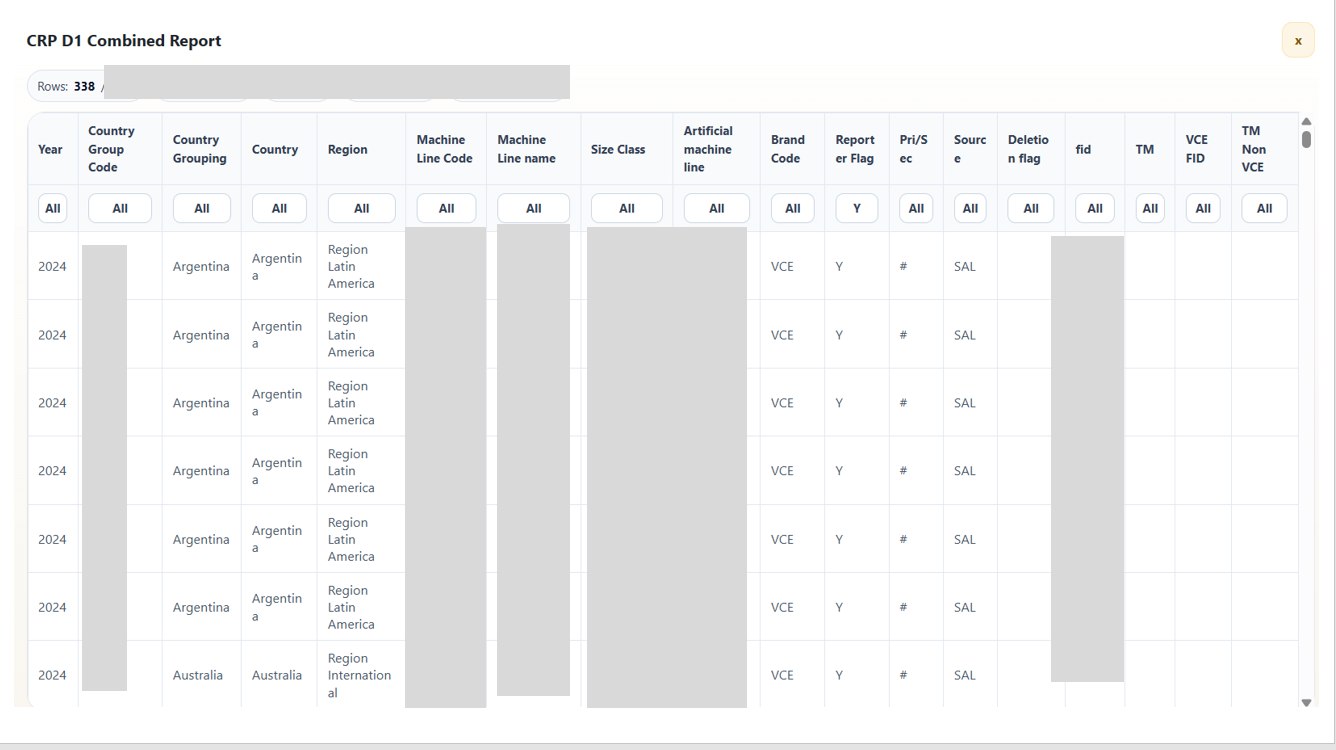
\includegraphics[width=1.1\linewidth]{6.1.png}
    \caption{CRP preparation validation result}
    \label{fig:crp_preparation_validation}
\end{figure}

\begin{figure}[H]
    \centering
    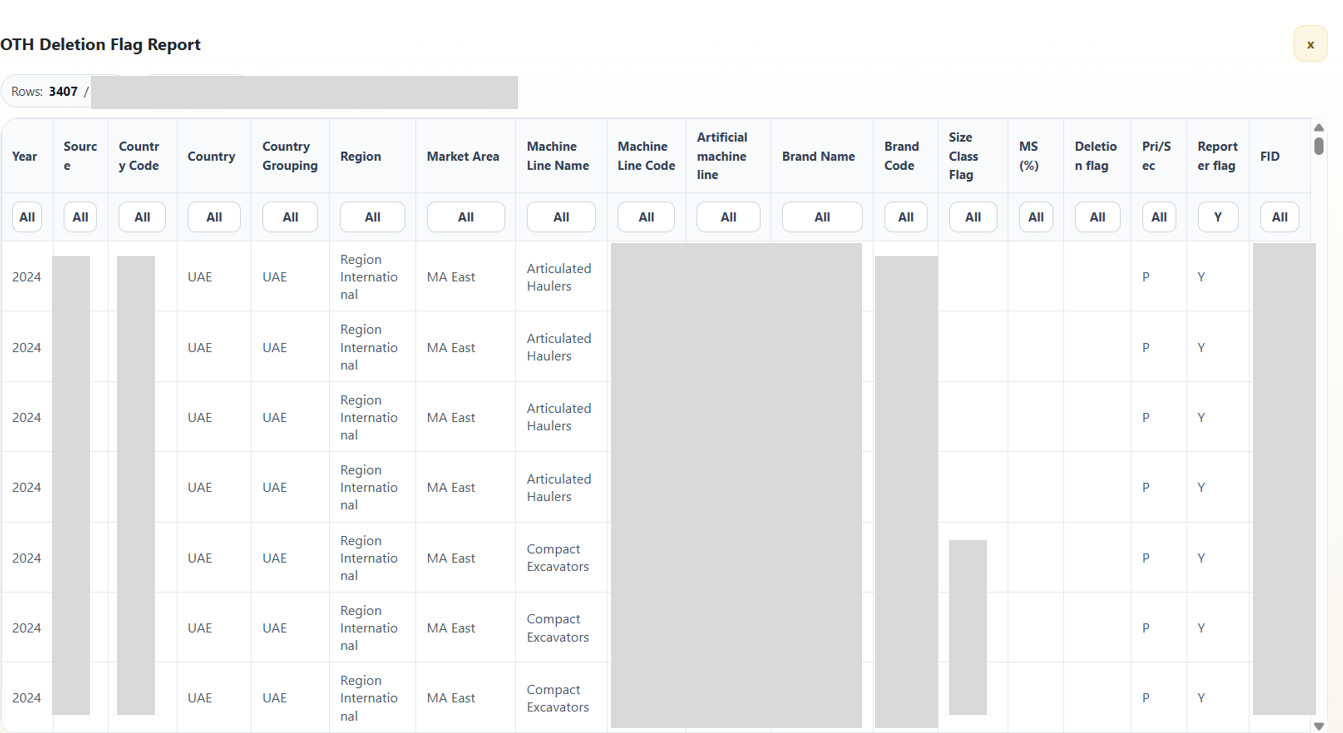
\includegraphics[width=1.1\linewidth]{6.2.png}
    \caption{OTH deletion flag and reporter flag validation result}
    \label{fig:oth_deletion_report_validation}
\end{figure}



\subsection{Split- and Resplit-Related Validation}

The split- and resplit-related outputs were validated through manual Excel-based checks, SAP reference comparison, and output inspection. For split validation, records that should enter the split process were manually filtered in Excel and compared with the prototype's split input totals. The totals were consistent for the tested Excavators and Wheel Loaders split cases, indicating correct record selection.

Approximately 10\% of split output rows and 10\% of resplit output rows were then spot-checked across selected country, source, machine-line, and size-class combinations. The sampled records followed the intended split and resplit logic, and the before/after totals remained consistent. Some differences from SAP outputs were nevertheless observed. Part of that difference was again related to reporter-list version differences, while one reviewed case suggested a different split-ratio basis in SAP than in the prototype. These findings were treated as reference-data and rule-clarification issues rather than direct prototype failures. Overall, the split and resplit logic behaved correctly within the tested scope.

\begin{figure}[H]
    \centering
    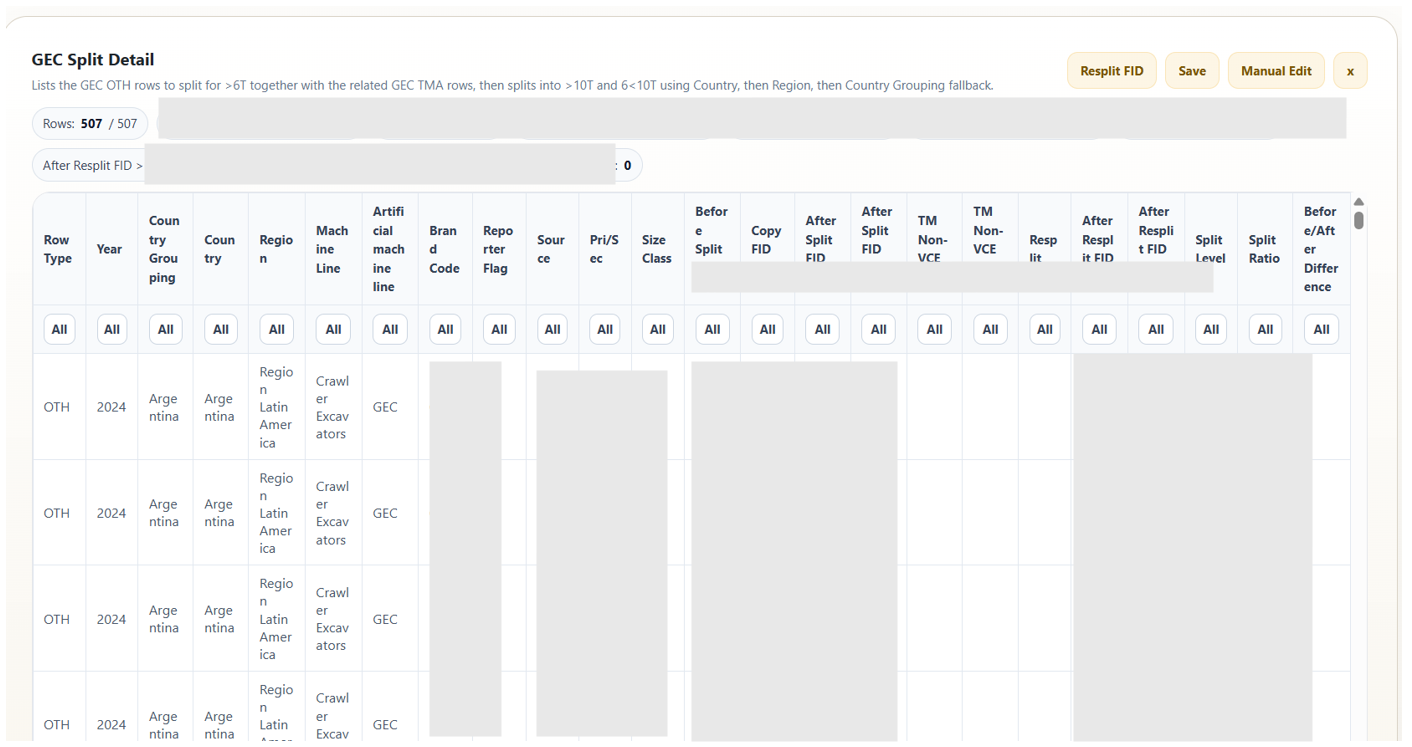
\includegraphics[width=1.1\linewidth]{6.3.png}
    \caption{Example of split and resplit validation results for GEC records}
    \label{fig:gec_split_resplit_validation}
\end{figure}

% \subsection{Summary of Validation Evidence and Results}

% Table~\ref{tab:data_evidence_validation} summarises the main validation evidence and results from the tested 2024 workflow data.

% \begin{longtable}{|>{\raggedright\arraybackslash}p{3.6cm}|>{\raggedright\arraybackslash}p{4.1cm}|>{\raggedright\arraybackslash}p{6.2cm}|}
% \caption{Summary of validation evidence and results}
% \label{tab:data_evidence_validation} \\
% \hline
% \textbf{Validation Area} & \textbf{Evidence / Data Checked} & \textbf{Validation Result} \\
% \hline
% \endfirsthead

% \hline
% \textbf{Validation Area} & \textbf{Evidence / Data Checked} & \textbf{Validation Result} \\
% \hline
% \endhead

% Preparation control flags & CRP reporter rows: 338; OTH reporter-flag rows: 3,407. & Reporter-related preparation outputs matched the expected classifications and corresponding SAP reference results. \\
% \hline

% Mapped fields & Country, market area, and related mapped fields checked against SAP export tables. & The mapped fields were aligned with the SAP-generated values in the tested 2024 data. \\
% \hline

% Market-view calculation & Approximately 20\% of rows sampled across selected country and machine-line combinations. & The sampled records showed correct TMA reduction by Volvo CE sales and correct VCE / Non-VCE ratio calculation. \\
% \hline

% Split and resplit outputs & Split-row selection and approximately 20\% of split/resplit rows sampled. & Split levels, split ratios, redistributed values, and before/after totals were consistent with expected rules in the sampled cases. \\
% \hline

% Runtime observation & Demonstration runs across preparation, market-view, adjustment, and split/resplit stages. & The prototype completed the tested runs within practical review time for prototype-level evaluation. \\
% \hline

% Stability observation & Repeated upload, run, filter, save/reload, and export cycles. & No crash, data loss, or inconsistent save/reload behaviour was observed in the tested scope. \\
% \hline

% \end{longtable}

% \section{Evaluation Against Requirements}

% The artefact was further evaluated against the requirements defined in Section~\ref{sec:requirements}. Each requirement was linked to an evaluation parameter and assessed using prototype functions, generated outputs, validation checks, runtime/stability observations, and stakeholder feedback.

% SAP reference outputs were used where direct comparison was possible, mainly for preparation-, split-, and resplit-related validation. Transparency, traceability, and usability were evaluated through prototype functions, visible intermediate outputs, available source/rule context fields, and stakeholder feedback. Performance and stability were assessed through observed execution and repeated review operations.

% The results are summarised in Table~\ref{tab:evaluation_parameters}.

% \begin{longtable}{|>{\raggedright\arraybackslash}p{1.2cm}|>{\raggedright\arraybackslash}p{2.7cm}|>{\raggedright\arraybackslash}p{4.0cm}|>{\raggedright\arraybackslash}p{6.0cm}|}
% \caption{Evaluation against requirements}
% \label{tab:evaluation_parameters} \\
% \hline
% \textbf{ID} & \textbf{Evaluation Dimension} & \textbf{Evaluation Parameter} & \textbf{Evaluation Result} \\
% \hline
% \endfirsthead

% \hline
% \textbf{ID} & \textbf{Evaluation Dimension} & \textbf{Evaluation Parameter} & \textbf{Evaluation Result} \\
% \hline
% \endhead

% FR1 & Functional fulfilment & Completion of source and matrix file upload and management. & Source and matrix files were uploaded, stored, displayed, downloaded, and reused across downstream stages. \\
% \hline

% FR2 & Functional fulfilment & Successful execution of backend workflow processing. & Backend processing executed preparation, adjustment, and split/resplit logic and produced outputs used for rule and SAP-reference validation. \\
% \hline

% FR3 & Functional fulfilment / usability & Availability of frontend review functions. & Filterable tables, summaries, charts, and CSV export supported browser-based review of detailed and aggregated outputs. \\
% \hline

% SR1 & Structural fit & Separation of upload, processing, storage, and visualisation components. & The artefact used a modular frontend-backend-database architecture with separated responsibilities. \\
% \hline

% SR2 & Structural fit & Structured storage of uploaded files, mappings, workflow records, and generated outputs. & Structured persistence supported repeated review, save/reload behaviour, and extension to later workflow stages. \\
% \hline

% PR1 & Performance & Successful completion of stage and report execution for the selected 2024 dataset. & Demonstration runs completed successfully across preparation, market-view, adjustment, and split/resplit flows. Observed execution time was typically within a few seconds and up to around one minute depending on stage complexity and row volume; formal production benchmarking was outside the thesis scope. \\
% \hline

% PR2 & Performance / stability & Absence of crashes, data loss, or inconsistent save/reload behaviour during repeated operations. & Repeated upload, run, filter, save/reload, and export cycles were executed during demonstration and validation. No crash, data-loss event, or inconsistent save/reload behaviour was observed in the tested 2024 scope. \\
% \hline

% QR1 & Transparency & Visibility of intermediate workflow stages, row-level outputs, and stage summaries. & Stage-specific views and outputs, including OTH deletion base, preparation, adjustment, and split/resplit, allowed stepwise inspection of how values were formed from one stage to the next. \\
% \hline

% QR2 & Traceability & Availability of source, mapping, control-flag, and rule-decision context in generated stage outputs. & Generated tables included source, country, machine line, artificial machine line, brand, reporter/deletion flags, split level, and split ratio fields, enabling stage-level traceability between uploaded inputs, applied rules, and resulting outputs. \\
% \hline

% QR3 & Usability & Ability to complete BI review tasks through the browser interface with acceptable effort. & Users completed review tasks through browser navigation, table filtering, summary/chart inspection, and CSV export. Stakeholder feedback indicated that these functions improved practical review compared with the prior representation. \\
% \hline

% ER1 & Environmental fit & Operation in a controlled prototype environment. & The artefact ran as a browser-accessible prototype with web frontend, backend service, and relational database for demonstration and evaluation. \\
% \hline

% ER2 & Environmental fit & Future adaptability to more robust cloud or Volvo CE internal infrastructure. & The modular design supports future adaptation to cloud or Volvo CE internal infrastructure; full enterprise integration remains future work. \\
% \hline

% \end{longtable}











% \section{Evaluation Against Requirements}

% The artefact was evaluated against the requirements defined in Section~\ref{sec:requirements}. Each requirement was assessed through generated outputs, SAP reference comparisons where applicable, runtime observations, repeated stability testing, and stakeholder feedback. Five repeated workflow runs with the selected 2024 dataset were used to record execution times for the main workflow stages.

% Stakeholder feedback was collected during prototype demonstrations and review discussions with Business Intelligence-related stakeholders in Volvo CE Strategy and Business Development, focusing on whether the separated workflow views, filters, summaries, and intermediate outputs made the selected TMC stages easier to inspect, validate, and discuss than in the SAP-based representation.

% The results are summarised in Table~\ref{tab:evaluation_parameters}.

% \begin{longtable}{|>{\raggedright\arraybackslash}p{3.2cm}|>{\raggedright\arraybackslash}p{4.6cm}|>{\raggedright\arraybackslash}p{6.2cm}|}
% \caption{Evaluation against requirements}
% \label{tab:evaluation_parameters} \\
% \hline
% \textbf{Requirement} & \textbf{Evaluation Question / Metric} & \textbf{Evidence and Result} \\
% \hline
% \endfirsthead

% \hline
% \textbf{Requirement} & \textbf{Evaluation Question / Metric} & \textbf{Evidence and Result} \\
% \hline
% \endhead

% FR1 Functional fulfilment & Can required source and matrix files be uploaded, shown, downloaded, and reused? & Yes. The required datasets in scope were uploaded and reused in workflow execution, including Source Matrix, Reporter List, Size Class, Brand Mapping, Group Country, Machine Line Mapping, OTH, CRP- and TMA-related data, and Volvo CE sales data. Upload pages supported \textit{Show Latest} and \textit{Download Latest}. \\
% \hline

% FR2 Functional fulfilment & Can backend logic generate staged workflow outputs? & Yes. The backend generated OTH deletion and reporter base outputs, preparation outputs, market-view outputs, adjustment outputs, and split/resplit outputs used in later validation. \\
% \hline

% FR3 Functional fulfilment / usability & Can users inspect outputs through frontend review functions? & Yes. Users reviewed outputs through filterable tables, summary cards, chart-based views, and CSV export. These functions were used in demonstration and validation tasks. \\
% \hline

% SR1 Structural fit & Are upload, processing, storage, and visualisation modularised? & Yes. The prototype operated with separated frontend pages, backend report and processing routes, and relational storage for uploaded and derived records. \\
% \hline

% SR2 Structural fit & Is workflow data persisted in structured form for repeated review? & Yes. Uploaded files, mapping data, intermediate records, and generated outputs were persisted and reused across stages, including repeated save/reload review cycles. \\
% \hline

% PR1 Performance & Can the 2024 workflow be completed within the defined 40-minute review window? & The selected 2024 workflow was tested \textbf{five} times and completed within the defined \textbf{40-minute} review window. The observed time ranges were approximately \textbf{4--5 minutes} for \textit{Upload Submit Matrix}, \textbf{5--6 minutes} for \textit{Upload OTH Data} and \textit{Upload CRP Data}, \textbf{10 minutes} for the preparation stage, \textbf{3 minutes} for the adjustment layer, and \textbf{10--12 minutes} for the machine line split layer. The workflow completion time included processing, result inspection, manual correction, and saving. \\
% \hline

% PR2 Performance / stability & Is behaviour stable during repeated upload, run, filter, save, reload, and export cycles? & The stability requirement was met during repeated validation runs. The prototype was tested through \textbf{five} repeated operation cycles using the selected 2024 dataset. Each cycle covered matrix upload, OTH/CRP upload, preparation, adjustment, machine line split, filtering, manual correction, saving, reload, and CSV export. The average completion time for a full workflow cycle was approximately \textbf{33 minutes}, remaining within the defined 40-minute review window. No crash, data loss, or inconsistent save/reload behaviour was observed. \\
% \hline

% QR1 Transparency & Are intermediate stages directly inspectable? & Yes. Stage outputs were visible separately, including OTH deletion base, preparation, adjustment, market view, and split/resplit, with row-level tables and summaries for stepwise inspection. \\
% \hline

% QR2 Traceability & Can output rows be related to source and rule context at stage level? & Partly. Outputs retained key context fields, including source, country, machine line, artificial machine line, brand, reporter/deletion flags, split level, and split ratio. This enabled stage-level tracing. Full end-to-end row lineage remains future work. \\
% \hline

% QR3 Usability & Can BI users complete review, validation, and export tasks with acceptable effort? & Yes within the prototype scope. Stakeholders could navigate stages, apply filters, inspect summaries/charts, and export CSV. Review feedback indicated improved practical inspectability compared with the prior representation. \\
% \hline

% QR4 Validation support & Do outputs match SAP and business-rule expectations where comparison is possible? & 
% Mostly yes.
% \begin{itemize}[leftmargin=*]
%     \item Manual Excel checks confirmed that the prototype applied the predefined rules correctly before comparison with SAP reference data. CRP reporter rows matched the SAP result, with 338 rows identified.
%     \item For OTH, the prototype classified 3,452 reporter rows, while SAP contained 3,467 rows with a net FID difference of 68. This was traced to a reporter-list version difference rather than a prototype error.
%     \item About 20\% of market-view rows and 10\% of split/resplit rows were spot-checked. The sampled records were consistent with expected calculations, split-case selection, redistribution logic, and before/after total preservation. One split-ratio discrepancy was recorded as a rule-clarification finding.
% \end{itemize}
% \\
% \hline

% ER1 Environmental fit & Can the artefact run in a controlled prototype environment? & Yes. The system was evaluated as a browser-accessible prototype with frontend, backend service, and relational database using 2024 workflow data. \\
% \hline

% ER2 Environmental fit & Is future adaptation to cloud or internal infrastructure feasible? & Partly. The modular design supports adaptation to cloud or Volvo CE internal infrastructure, but enterprise integration, production deployment, and internal authentication/integration constraints remain future work. \\
% \hline

% \end{longtable}




\subsection{Evaluation Against Requirements}

The artefact was evaluated against the functional and performance requirements defined in Section~\ref{sec:requirements}. The assessment combined generated workflow outputs, SAP reference comparisons where applicable, manual Excel checks, runtime observations, repeated stability testing, and stakeholder feedback from weekly review discussions.

Overall, the results indicate that the main requirements were met within the prototype scope. The system supported upload and reuse of the required datasets, generated staged outputs for the selected workflow layers, and provided structured inspection through filters, summaries, charts, and CSV export. Validation support was also largely confirmed: manually checked rule behaviour matched the prototype outputs, CRP reporter rows matched the SAP reference result, and sampled market-view and split/resplit records followed the expected calculation logic. The main observed exception was an OTH reporter-row difference that was traced to a reporter-list version difference rather than a prototype error.

Performance and stability results were also acceptable for the evaluated setting. Repeated workflow cycles remained within the defined review window, and no crash, data loss, or inconsistent save/reload behaviour was observed during the repeated test runs. A more detailed requirement-by-requirement table is provided in Appendix~\ref{app:supplementary-material}.








% \section{Comparison with the SAP-Based Workflow}

% To further clarify transparency, traceability, usability, and validation support, the prototype was compared with the SAP-based workflow from a business-user perspective. The comparison does not claim that SAP lacks these capabilities technically, but assesses whether they are directly available and inspectable for business users within the reviewed workflow.

% \begin{longtable}{|>{\raggedright\arraybackslash}p{2.8cm}|>{\raggedright\arraybackslash}p{2.5cm}|>{\raggedright\arraybackslash}p{2.5cm}|>{\raggedright\arraybackslash}p{5.8cm}|}
% \caption{Concise comparison between SAP-based representation and prototype}
% \label{tab:sap_prototype_comparison} \\
% \hline
% \textbf{Dimension} & \textbf{SAP-based Workflow} & \textbf{Prototype} & \textbf{Evidence in this thesis} \\
% \hline
% \endfirsthead

% \hline
% \textbf{Dimension} & \textbf{SAP-based Workflow} & \textbf{Prototype} & \textbf{Evidence in this thesis} \\
% \hline
% \endhead

% Transparency & Limited for business-user inspection & Supported & Preparation, adjustment, and split/resplit are exposed as separate inspectable stages with row-level and summary views. \\
% \hline

% Traceability & Limited and dispersed across technical structures & Partly supported & Stage outputs preserve source/rule context fields, including country, machine line, source, brand, flags, split level, and split ratio, enabling stage-level tracing. \\
% \hline

% Usability & Requires more SAP-specific navigation & Supported & Browser-based filtering, summaries/charts, and CSV export supported practical BI review tasks. \\
% \hline

% Validation support & Often requires extra extraction or IT support & Supported & Intermediate values, totals, and split parameters were directly inspectable and comparable with expected rules and SAP references. \\
% \hline

% \end{longtable}



\section{Comparison with the SAP-Based Workflow}

To further clarify transparency, traceability, usability, and validation support, the prototype was compared with the SAP-based workflow from a business-user perspective. The comparison does not claim that SAP lacks these capabilities technically, but assesses whether they are directly available and inspectable for business users within the reviewed workflow.

Compared with the SAP-based representation, the prototype made four differences visible within the evaluated scope. First, transparency improved because preparation, adjustment, and split/resplit outputs were exposed as separate inspectable stages rather than being dispersed across technical SAP artefacts. Second, traceability improved at stage level because outputs retained source and rule context such as country, machine line, source, brand, flags, split level, and split ratio. Third, usability improved because business users could review results through browser-based filtering, summaries, charts, and CSV export rather than SAP-specific navigation. Fourth, validation became more direct because intermediate values and rule-relevant fields could be inspected without additional extraction or IT-supported investigation.








% \section{Summary and Limitations}

% The evaluation showed that the artefact fulfilled its core purpose as a web-based prototype for the selected TMC workflow stages. Within the implemented scope, it supported structured CSV upload, staged backend processing, workflow-layer inspection, and validation against 2024 SAP reference results and expected business rules. It also supported transparency, stage-level traceability, usability, validation support, and prototype-level performance in the controlled test setting.

% Several limitations nonetheless apply:
% \begin{itemize}
% \item The prototype covers only selected stages of the broader TMC process, and the formal evaluation scope was limited to outputs up to machine line split/resplit.
% \item The validation was conducted with data from the 2024 calculation cycle, so the results cannot yet be generalised across all years and workflow variations.
% \item The artefact supports stage-level traceability, but full row-level lineage across all transformations remains future work.
% \item The artefact remains sensitive to the structural quality of uploaded CSV files and mapping data, despite the cleaning and normalisation logic that has been implemented.
% \item The current deployment and storage setup is adequate for prototype use, but broader internal deployment would require more robust infrastructure and deeper integration with enterprise systems.
% \end{itemize}

\section{Summary and Limitations}

The evaluation showed that the artefact fulfilled its core purpose as a web-based prototype for the selected TMC workflow stages. Within the implemented scope, it supported structured CSV upload, staged backend processing, intermediate output inspection, and rule-based validation against 2024 SAP reference outputs where comparison was possible. The results indicate that the prototype improved transparency and stage-level traceability by making preparation, market-view, adjustment, and split/resplit outputs easier to inspect and verify.

The validation results were largely consistent with the expected business rules. CRP preparation matched the SAP reference output, while the observed OTH reporter-flag difference was traced to a reporter-list version difference rather than a prototype error. For split and resplit, Excel-based checks showed that totals were preserved and sampled records followed the expected split-case, redistribution, and size-class flag rules. One split-ratio difference was identified as a rule-clarification issue.

Several limitations nonetheless apply:
\begin{itemize}
    \item The prototype covers only selected stages of the broader TMC process. Formal evaluation was limited to source upload, preparation, market-view derivation, adjustment, and selected split/resplit-related outputs.
    \item The validation was based on the 2024 calculation cycle, so the findings cannot yet be generalised to all years, source configurations, or annual workflow variations.
    \item Some SAP comparisons were affected by reference-data or calculation-basis differences, such as the reporter-list adjustment and the observed split-ratio discrepancy.
    \item The artefact supports stage-level traceability, but full row-level lineage across all transformations remains future work.
    \item The current deployment and storage setup is adequate for prototype demonstration, but broader internal use would require more robust infrastructure, access control, and integration with enterprise systems.
\end{itemize}
